\subsection{Far-field scattering} \label{sec:ff_scattering}


\begin{figure}[h] %  figure placement: here, top, bottom, or page
   \centering
   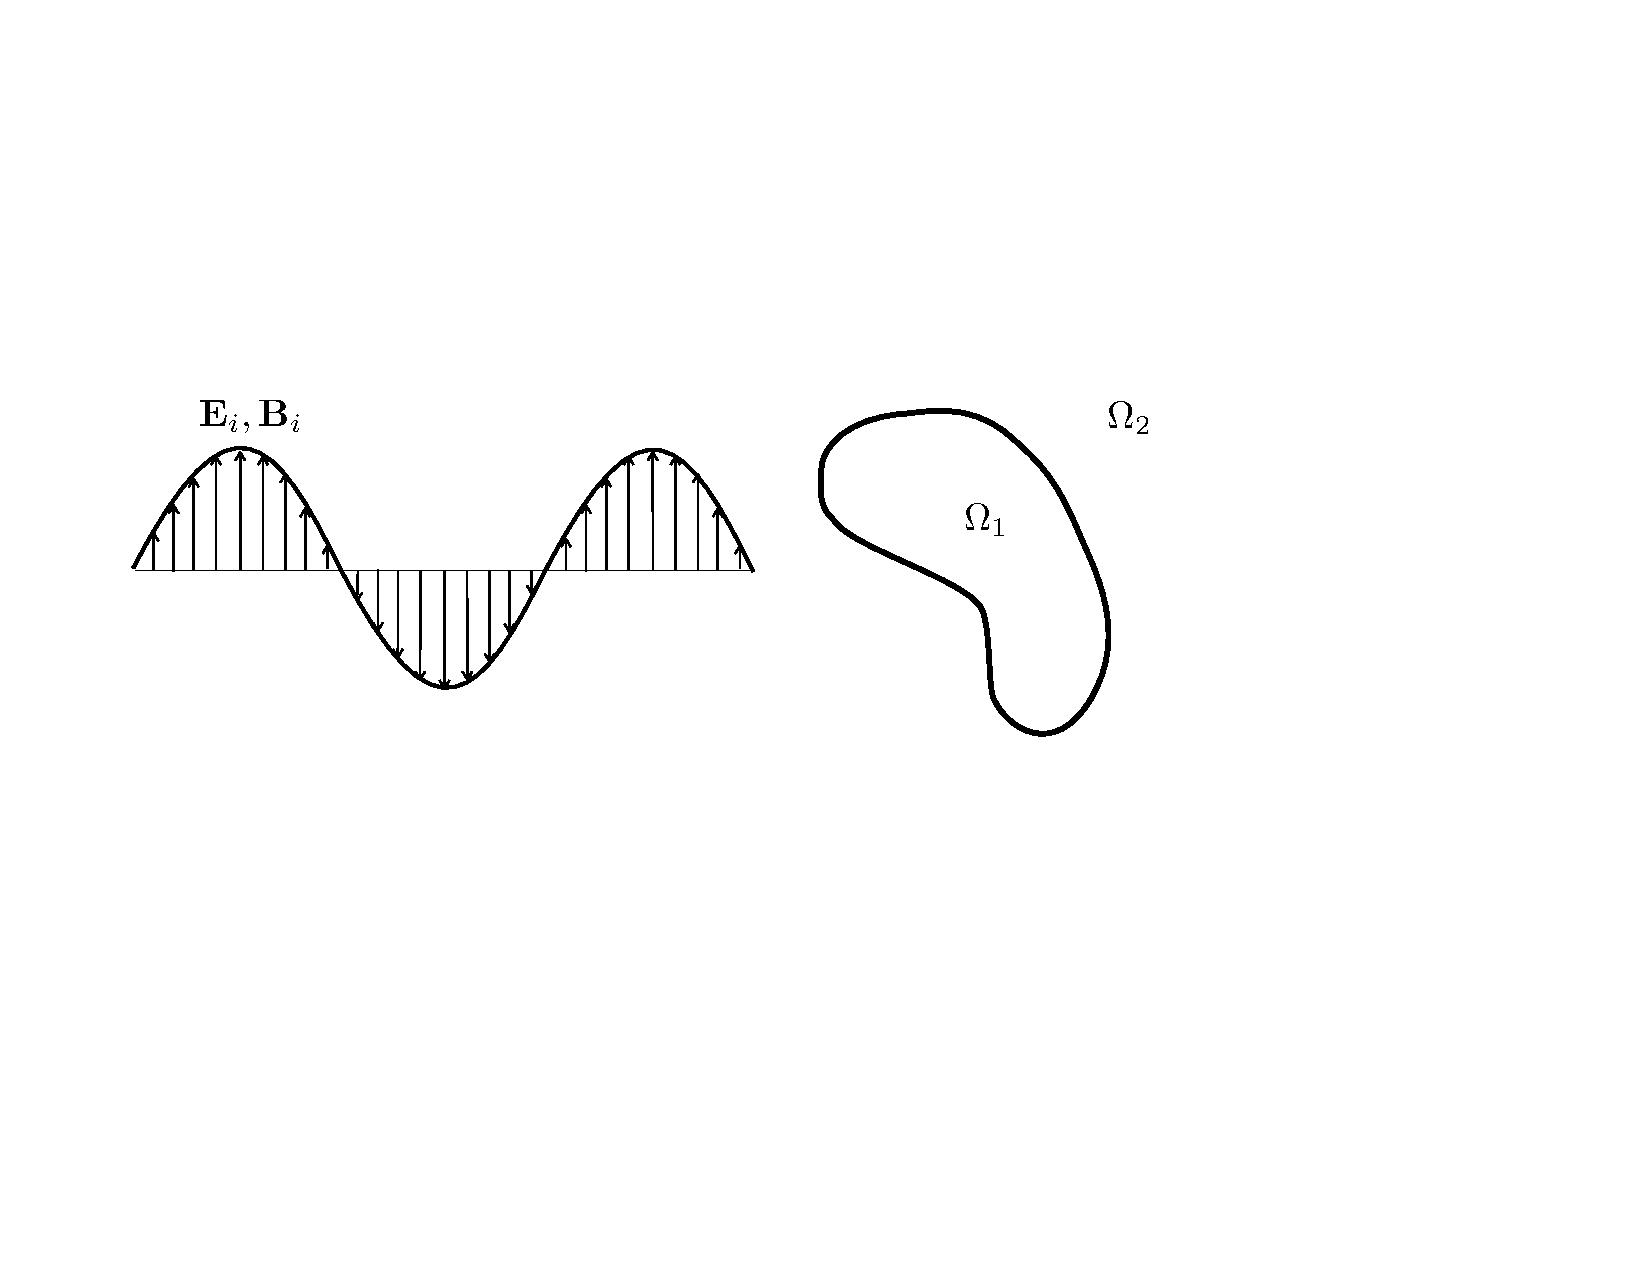
\includegraphics[width=0.45\textwidth]{particle_wave.pdf} 
   \caption{Nanoparticle under electromagnetic wave.}
   \label{fig:part_wave}
\end{figure}

In LSPR computations, we measure the scattered electromagnetic field on a detector
that is located far away from the nanoparticle. When light shines on an object 
like in Figure \ref{fig:part_wave}, the incident wave ($\mathbf{E}_i$,  $\mathbf{B}_i$)
is scattered along the domain, resulting in a total electromagnetic field 
($\mathbf{E}$,  $\mathbf{B}$) that depends on the incoming wave, the particle's 
geometry, and the material constants. In the quasistatic approximation, we only
 need to compute the electric field and the magnetic contribution can be 
neglected \cite{MayergoyzZhang2007}. In the far-field limit, the scattered field
in the outside region ($\Omega_2$) is given by: 

\begin{equation} \label{eq:scat_efield_long_range}
    \mathbf{E}_{2s} = \frac{1}{4\pi\epsilon_2}k^2\frac{e^{ikr}}{r} (\mathbf{\hat{r}} \times \mathbf{p})\times\mathbf{\hat{r}}.
\end{equation} 

where $k=2\pi/\lambda$ is the wave number and $\lambda$ the wavelength, $\mathbf{\hat{r}}$ 
is a unit vector in the direction of the observation point, and $\mathbf{p}$ is
the dipole moment.

We can also obtain the scattered field with the forward-scattering amplitude 
\cite{Jackson}:

\begin{equation} \label{eq:scat_efield_fwa}
    \mathbf{E}_{2s}(\mathbf{r})_{r\to\infty} = \frac{e^{ikr}}{r} \mathbf{F}(\mathbf{k},\mathbf{k}_0),
\end{equation}

where $\mathbf{F}$ is the forward-scattering amplitude, $\mathbf{k}$ is the 
scattered wave vector in the direction of propagation, and $\mathbf{k}_0$ the 
wave vector of the incident field. 

Via these two equations, we use \pygbe to compute the scattered electric field 
and then solve for the forward-scattering amplitude. 

\subsection{Extinction cross-section and Optical theorem} \label{sec:cext_ot}

The extinction cross-section quatifies how much extinction (scattered + absorbed) 
is caused by a particle when this one is shinned with light. It is defined as the
ratio between the extinct energy and the intensity of the incoming wave. 

The optical theorem relates the extinction cross-section with the forward-scattering amplitude. The traditional expression for this relationship applies for non-absorbing media \cite{MayergoyzZhang2007, Jackson}. The expression for absorbing media \cite{BohrenGilra1979, VideenSun2003} was corrected by Mishchenko \cite{Mishchenko2007}, giving the following expression:

\begin{equation} \label{eq:cext_fwa}
    C_\text{ext} = \frac{4\pi}{k^\prime} \operatorname{Im} \left[ \frac{\mathbf{\hat{e}}_i}{|\mathbf{E}_i|}\mathbf{F}(\mathbf{k}=\mathbf{k}_0, \mathbf{k}_0) \right].
\end{equation}


{\color{red}{Chris in Mishenko 2007 paper the equation is not exactly the same 
(look eq 87 in paper), do you have that derivation? How you got to the eq 7.22 
 in your thesis?.}}


Here, $k^\prime$ is the real part of the complex wave number. 

\begin{equation}
    k = k^\prime + ik^{\prime\prime} = \frac{2\pi}{\lambda} n,
\end{equation}

and $n$ is the refraction index of the host medium.


\subsection{Boundary integral formulation} \label{sec:lspr_bem}

From the electrostatic approximation from Mayergoyz and Zhang (2007) 
\cite{MayergoyzZhang2007} we know that the zeroth order term of the magnetic 
field is zero everywhere. Resulting in the following Maxwell equations. 

\begin{align} \label{eq:electrostatic_scatter_E}
\nabla \cdot \mathbf{E}^{(0)}_{1s} &= 0 \qquad \nabla \times \mathbf{E}^{(0)}_{1s} = 0 \nonumber \\
\nabla \cdot \mathbf{E}^{(0)}_{2s} &= 0 \qquad \nabla \times \mathbf{E}^{(0)}_{2s} = 0 \nonumber \\
(\epsilon_1\mathbf{E}^{(0)}_{1s} - \epsilon_2\mathbf{E}^{(0)}_{2s})\cdot\mathbf{n} &= (\epsilon_2-\epsilon_1)\mathbf{E}_i\cdot \mathbf{n}.
\end{align}

Where the subscript $s$ ($i$) stands for scattered (incident) field. The curl of
$\mathbf{E}^{(0)}_{js}$ for $j=1,2$ is zero, therefore, there is a scalar potential
such that $-\nabla \phi_js = \mathbf{E}^{(0)}_js$. Using this, we can rewrite 
equation \ref{eq:electrostatic_scatter_E} as:

\begin{align} \label{eq:electrostatic_scatter}
\nabla^2 \phi_{1s} &= 0 \qquad \nabla^2 \phi_{2s} = 0 \qquad\text{on $\Omega_1$, $\Omega_2$} \nonumber \\
\epsilon_1\frac{\partial\phi_{1s}}{\partial \mathbf{n}} - \epsilon_2\frac{\partial\phi_{2s}}{\partial\mathbf{n}} &= (\epsilon_2-\epsilon_1)\frac{\partial\phi_i}{\partial\mathbf{n}} \qquad \phi_{1s} = \phi_{2s} \qquad\text{on the boundary $\Gamma$}.
\end{align}


Recalling the weak formulation of Laplace equation with test function $w$:

\begin{equation} \label{eq:lap_weak}
\int_\Omega \nabla^2 \phi(\mathbf{r}_\Omega') w(\mathbf{r}_\Omega') \text{d} \Omega^\prime= 0.
\end{equation}

where the evaluation point is $\mathbf{r}_\Omega$ a location in the domain $\Omega$.

If we use the Laplace's free-space Green's function as the test function $w$ we
get:

\begin{equation} \label{eq:lap_weak2}
\int_\Omega \nabla^2 \phi(\mathbf{r}'_\Omega) G_L(\mathbf{r}_\Omega,\mathbf{r}'_\Omega) \text{d} \Omega^\prime= 0.
\end{equation}




\subsubsection{Electrostatic potential under an incoming electric field}


\subsubsection{Boundary integral expression of the dipole moment}

\subsection{Acceleration startegies} \label{sec:acc_strategies}













